\chapter{Data and Descriptive Statistics} \label{Chap3}
This chapter provides a meticulous analysis of the dataset, focusing on the Euro currency market in the EMEA region. Key variables like Censor Status, Deal Value, Cover Price, and Reference Price are defined. Sector distribution and price patterns are visually explored, offering valuable insights. These analyses form the groundwork for the subsequent in-depth examination and modeling in the following chapters.

\section{Data Source and Selection}
The dataset for this study was sourced from the Hydra database, a Python database package utilized at JPMC, covering the period from February 6th, 2023, to June 19th, 2023. Data importation occurred weekly, ensuring an up-to-date and comprehensive dataset. Encompassing 11 distinct financial sectors, the financial sector stood out with a significant volume of Request for Quotes (RFQs), while the diversified sector had fewer RFQs.

During the data selection process, specific criteria were applied to ensure dataset relevance and appropriateness.

\subsection{Currency}
The dataset includes various currencies:

\begin{itemize}
    \item \textbf{AUD:} Australian Dollar
    \item \textbf{USD:} United States Dollar
    \item \textbf{EUR:} Euro
    \item \textbf{GBP:} British Pound Sterling
    \item \textbf{NOK:} Norwegian Krone
    \item \textbf{DEM:} German Mark (historical currency)
    \item \textbf{NLG:} Dutch Guilder (historical currency)
    \item \textbf{CHF:} Swiss Franc
    \item \textbf{HUF:} Hungarian Forint
    \item \textbf{SEK:} Swedish Krona
    \item \textbf{JPY:} Japanese Yen
    \item \textbf{CNY:} Chinese Yuan
    \item \textbf{ITL:} Italian Lira (historical currency)
    \item \textbf{CAD:} Canadian Dollar
    \item \textbf{ZAR:} South African Rand
    \item \textbf{BRIL:} Brazilian Real
    \item \textbf{DKK:} Danish Krone
    \item \textbf{HKD:} Hong Kong Dollar
    \item \textbf{MXN:} Mexican Peso
    \item \textbf{SGD:} Singapore Dollar
    \item \textbf{ILS:} Israeli New Shekel
    \item \textbf{FRF:} French Franc (historical currency)
\end{itemize}

However, for the purpose of this analysis, the focus is exclusively on the Euro (EUR) currency. By concentrating on EUR, the study achieves a targeted analysis, allowing for a comprehensive and detailed examination within the specific context of the Euro currency market.

\subsection{Direction}
First and foremost, the direction of RFQs was considered. The dataset contained both buy and sell RFQs. However, the analysis focused exclusively on buy-side RFQs. This decision was motivated by the asymmetrical nature of responses to sell-side RFQs, which introduced complexities that were not conducive to the scope of this study.

\subsection{Region}
There are four global regions covered in the dataset:

\begin{itemize}
    \item \textbf{EMEA:} Europe, Middle East, and Africa.
    \item \textbf{APAC:} Asia and Pacific regions.
    \item \textbf{LATAM:} Latin America.
    \item \textbf{NA:} North America, including the USA and Canada.
\end{itemize}

For this analysis, the focus is solely on the EMEA market data. This specific focus on the EMEA region is driven by the study's emphasis on the Euro currency market within Europe. By concentrating on the Eurozone, the analysis gains a targeted perspective on a specific and significant currency market, allowing for a more in-depth and nuanced examination of RFQs within this specific monetary context.

\subsection{Status}
Additionally, the dataset included RFQs with various statuses:

\begin{enumerate}
    \item \textbf{REJECTED\_DEALER:} The market maker rejected the RFQ, opting not to proceed with the trade.
    \item \textbf{CANCELLED\_CLIENT:} The client initiated the cancellation of the RFQ, deciding not to proceed with the trade.
    \item \textbf{TIMEOUT\_DEALER:} The market maker took too long to respond to the RFQ, leading to a timeout situation where the trade did not proceed.
    \item \textbf{TRADE\_TRADEDAWAY:} The market maker did not win the trade. They were not the first or second best option for the client, resulting in the RFQ not being executed.
    \item \textbf{REJECTED\_CLIENT:} The client rejected the market maker's offer, choosing another option or not proceeding with the trade.
    \item \textbf{TRADE\_DONE:} A successful trade execution where the market maker won the trade, and the RFQ resulted in a transaction.
    \item \textbf{TIMEOUT\_CLIENT:} The client took too long to accept the market maker's price, leading to a timeout situation where the trade did not proceed.
    \item \textbf{TRADE\_COVERED:} The market maker was the exact second best option for the client, resulting in a covered trade where the RFQ was successfully executed.
    \item \textbf{TRADE\_COVEREDTIED:} The market maker was the second best option, but there was a tie with another participant at the same price. The trade was covered despite the tie.
    \item \textbf{TRADE\_TIEDTRADEDAWAY:} The market maker was not the first or second best option, and there was a tie with another participant at the same price. The RFQ did not result in a trade.
    \item \textbf{QUOTE\_CANCELLED:} The market maker responded to the price before the client could accept it, but the client canceled the RFQ, leading to a non-execution of the trade.
\end{enumerate}

However, only RFQs falling into 5 specific categories were utilized for analysis: \textit{TRADE\_\-TRADED\-AWAY}, \textit{TRADE\_DONE}, \textit{TRADE\_COVERED}, \textit{TRADE\_COVEREDTIED}, \textit{TRADE\_TIED\-TRADED\-AWAY}. These specific statuses were chosen due to their relevance to the study's objectives. They represented instances where the market maker was either successful in executing the trade, secured a covered trade position, or encountered tied situations, all of which were critical for the analysis of RFQ success rates.

This meticulous data selection process ensured that the dataset used for subsequent analysis was finely tuned, containing RFQs that provided valuable insights into the market maker's performance and success rates.

\section{Variables Definitions}
Let's delve into the definitions of key variables within the dataset. Understanding these variables will provide a comprehensive insight into the fundamental characteristics of my dataset.

\subsection{Censor Status}
Definition: Censor Status $c_i$ denotes the censor status of $i^{th}$ quote:

\[
c_i =
\begin{cases}
    1, & \textit{TRADE\_DONE}, \\
    0, & \textit{TRADE\_TRADEDAWAY,} \\
    0, & \textit{TRADE\_COVERED,} \\
    0, & \textit{TRADE\_COVEREDTIED,} \\
    0, & \textit{TRADE\_TIEDTRADEDAWAY}
\end{cases}
\]

In the context of my financial data, the definition of censor status aligns with traditional survival analysis principles. When a trade event doesn't occur within the study period, it's marked as uncensored (0) because the outcome isn't observed, akin to the standard survival analysis concept. Conversely, if a trade event occurs, it's censored (1) because the exact timing isn't always known, similar to right-censored events in survival analysis. The purpose of this definition is to be more consistent with the estimator formula of traditional survival analysis.

\subsection{Deal Value}
Definition: Deal Value $t^d_i$ denotes the successfully traded price of $i^{th}$ quote. "Traded price" refers to a situation where the market maker's quote was not only accepted but also chosen as the winning bid. In this scenario, the market maker successfully secured the transaction, and the price at which the trade was executed is termed the "traded price." This price represents the rate at which the market maker agreed to buy or sell the financial instrument with the client, indicating a successful transaction between us and the client.

\subsection{Cover Price}
Definition: Cover Price $t^c_i$ denotes the observed covered price of $i^{th}$ quote. The term "covered price" signifies a scenario where the market maker's initial quote was not accepted, but they happened to be the second-best option. In this situation, the system returns to us the price at which the trade was executed by the first-place bidder. This indicates that the market maker's quote was covered, or matched, at this particular price. Being covered in this context means that the transaction was successfully completed, even though the market maker's original quote was not directly accepted.

\subsection{Reference Price}
In financial datasets, multiple reference prices can exist because different market participants may use various data sources for pricing. The choice of reference price depends on the specific financial instrument being traded and market conventions. Institutions like Bloomberg and the London Stock Exchange (LSE) are common sources of reference prices in the financial industry. Bloomberg, for example, offers a wide range of financial data, including reference prices, market analysis, and trading insights. Similarly, the LSE provides market data services, including various pricing information relevant to financial instruments like bonds.

These institutions gather and provide comprehensive data to traders, investors, and financial analysts, serving as reliable sources for reference prices and other critical financial information. The choice of which institution to use often depends on the specific needs of the financial professionals and institutions accessing the data. Different entities might prefer different platforms based on factors like data accuracy, coverage, and user interface. In my research, I opted for Bloomberg as my primary data source due to its comprehensive and up-to-date datasets. Utilizing Bloomberg ensured the availability of the latest and most extensive data, providing a stable foundation for comparisons with my model.

Common data sources for reference prices include:
\begin{table}[H]
    \caption{Descriptions of Reference Price Terms. All terms are denominated in USD.}
    \label{tab:reference_price_terms}
    \begin{tabular}{|>{\centering\arraybackslash}m{2cm}|>{\centering\arraybackslash}m{7cm}|>{\centering\arraybackslash}m{4cm}|}
    \hline
    \textbf{Term} & \textbf{Definition} & \textbf{Usage} \\
    \hline
    Mid Price $t^m_i$ & The mid price in bond trading represents the average between the highest bid price (the price buyers are willing to pay) and the lowest ask price (the price sellers are willing to accept) of the $i^{th}$ bond trading quote. It's a fair estimate of the current market value. & Commonly used for bonds, indicating a balanced point between buy and sell interests. \\
    \hline
    Acceptable Price Range $t^r_i$ & An acceptable price range of the $i^{th}$ bond trading quote denotes a predefined span of prices within which a trade can occur. Trades falling within this range are considered valid and executable. & Provides flexibility and scale in bond trading, allowing trades within a specified price band. \\
    \hline
    Yield $t^y_i$ & Yield in bond trading represents the return on investment, calculated as the annual income earned from the bond of the $i^{th}$ trading quote relative to its price. It indicates the profitability of a bond investment. & Predominantly used for bonds, expressing the return on investment and influencing pricing decisions. \\
    \hline
    \end{tabular}
\end{table}

\subsection{Relative Price}
Definition: Relative price (Price) $t_i$ denotes the standardized price of $i^{th}$ quote:
\begin{align}
    t_i &= \frac{t^d_i - t^m_i}{t^r_i},\ c_i = 0,\notag \\
    &= \frac{t^c_i - t^m_i}{t^r_i},\ c_i = 1.\label{eq:p}
\end{align}

Formula \eqref{eq:p} standardizes quoted prices across different bonds, producing the relative price based on the reference price. Initially, I chose available prices: For completed quotes, the traded price $t^d_i$ is used, while for pending quotes, the cover price $t^c_i$ is utilized. The mid-price $t^m_i$ is subtracted from these values, and the result is divided by the corresponding acceptable price range $t^r_i$. This process enables us to concentrate on relative prices for various types of securities. Standardizing prices in this manner unifies the scale in subsequent estimators and mitigates the influence of different bonds on the estimator's performance.

I also dropped some quote that can't calculate $t_i$ here since there are some unusual scenarios, such as only one market maker sends quote but there doesn't exist the $2^{nd}$ competitor and some price are missed.

\section{Descriptive Statistics}
\subsection{Sector Distribution}
\begin{figure}[ht]
    \centering
    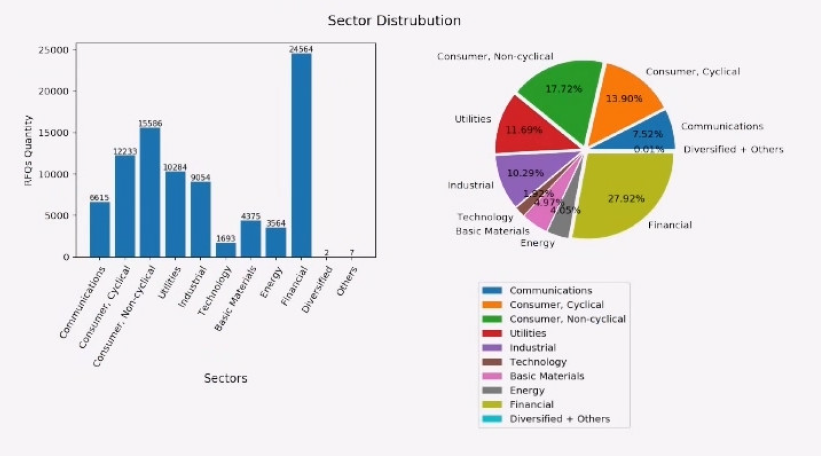
\includegraphics[width=0.8\textwidth]{figures/jpm/1. Sector Distribution.png}
    \caption{Sector Distribution}
    \label{fig:sector_distribution}
\end{figure}

This visualization employs both bar and pie charts to illustrate the quantity distribution of quotes across various sectors. In the smaller chart on the left, the x-axis represents different sectors, totaling 11: communications, consumer cyclical, consumer non-cyclical, utilities, industrial, technology, basic materials, energy, financial, diversified, and others. Notably, the financial sector stands out with a substantial quote count, exceeding 24,000. This high volume can be attributed to the extensive bond transactions and frequent trading activities within the financial industry. The top four sectors in terms of quotes are financial, followed by consumer sectors and utilities. In contrast, diversified and others have only 2 and 7 quotes, respectively, making them negligible in our analysis. Consequently, these two sectors will receive minimal focus in subsequent models.

\begin{figure}[H]
    \centering
    \includegraphics[width=0.8\textwidth]{figures/jpm/4. Heatmap of RFQs in test set.png}
    \caption{Heatmap of RFQs in Test Set}
    \label{fig:rfqs_heatmap_test}
\end{figure}

\begin{figure}[H]
    \centering
    \includegraphics[width=0.8\textwidth]{figures/jpm/5. Heatmap of RFQs that trade done in test set.png}
    \caption{Heatmap of RFQs with Trade Done in Test Set}
    \label{fig:rfqs_heatmap_trade_done_test}
\end{figure}

\begin{figure}[H]
    \centering
    \includegraphics[width=0.8\textwidth]{figures/jpm/6. Heatmap of real HR of RFQs in test set.png}
    \caption{Heatmap of Real HR of RFQs in Test Set}
    \label{fig:rfqs_heatmap_real_hr_test}
\end{figure}

These three heatmaps provide an alternative perspective on quotes across various industries and the distribution of transaction quotes over time. The vertical axis denotes time, divided into 15 intervals based on quote generation time, with single orders increasing from top to bottom (for detailed "fold" definitions, refer to \ref{Chap4}). The horizontal axis categorizes different sectors. The numbers within each square indicate the quantity of quotes, with darker colors representing higher numbers. \ref{fig:rfqs_heatmap_test} displays all quotes, \ref{fig:rfqs_heatmap_trade_done_test} shows trade done quotes, and \ref{fig:rfqs_heatmap_real_hr_test} presents the ratio of transaction quotes. These visuals reveal continuity in the previously observed distribution patterns. Notably, quotes are evenly spread across time intervals, and sectors with a significant proportion of quotes maintain a substantial share within each fold. Remarkably, the transaction proportion remains remarkably stable, consistently hovering around 0.1-0.2. 

An anomaly is observed in the transaction rate for the 'other' sector, recorded as 1.00 in the 9th fold. This irregularity stems from 2 quotes within this sector, leading to an unrealistic transaction rate. Given its abnormal nature and the fact that it comprises only 2 quotes that was successfully traded, this data point is considered an outlier and is disregarded in the analysis.

\subsection{Price Distribution}
\begin{figure}[ht]
    \centering
    \includegraphics[width=0.8\textwidth]{figures/jpm/2. Price Distribution.png}
    \caption{Price Distribution}
    \label{fig:price_distribution}
\end{figure}

In my final analysis, I examined the price distribution by generating a histogram. The x-axis represents the price, while the y-axis represents the number of quotes for each price point. To enhance visibility, two scales were utilized: a linear y-axis on the left and a logarithmic y-axis on the right. This dual representation was necessary to clearly discern the specific distribution of prices.

Observing the histogram, I noticed a concentration of prices on the negative half axis. The quantity of quotes increases as the prices approach the 0 point. This pattern aligns with my expectations as I primarily investigated bid quotes, where market makers aim to make profits with lower bids. Upon calculation, the mean price was found to be -1.04, with a variance of 2.01, validating my observations.

These meticulous data selections and analyses laid a solid foundation for the subsequent chapters' in-depth exploration and modeling.